
%=========================================================
% PARTIE 1.2 : CLASSIFICATION BAYESIENNE
%=========================================================

\section{Classification bayésienne}

\subsection{Calcul des probabilités bayésiennes}

L'objectif de cette étape est de déterminer, pour chaque
observation $\mathbf{x}(n)$, les probabilités d'appartenance
aux deux classes $E^+$ et $E^-$.

On définit le vecteur des probabilités par :

\begin{equation}
\mathbf{P}(n)=
\begin{bmatrix}
P_+(n)\\
P_-(n)
\end{bmatrix}
\end{equation}

avec :

\begin{equation}
P_+(n)=P(E^+\mid\mathbf{x}(n))
\end{equation}

et

\begin{equation}
P_-(n)=P(E^-\mid\mathbf{x}(n)).
\end{equation}

D'après la formule de Bayes, la probabilité a posteriori
d'une classe est donnée par :

\begin{equation}
P(E^\pm\mid\mathbf{x})=
\frac{p(\mathbf{x}\mid E^\pm)P(E^\pm)}
{p(\mathbf{x})}.
\end{equation}

Dans notre cas, les symboles transmis prennent les valeurs
$+1$ et $-1$ avec la même probabilité. Les probabilités
a priori des deux classes sont donc :

\begin{equation}
P(E^+)=P(E^-)=\frac{1}{2}.
\end{equation}

Par conséquent, les probabilités a posteriori deviennent :

\begin{equation}
P_+(\mathbf{x})=
\frac{p(\mathbf{x}\mid E^+)}
{p(\mathbf{x}\mid E^+)+p(\mathbf{x}\mid E^-)}
\end{equation}

et

\begin{equation}
P_-(\mathbf{x})=
\frac{p(\mathbf{x}\mid E^-)}
{p(\mathbf{x}\mid E^+)+p(\mathbf{x}\mid E^-)}.
\end{equation}

\subsubsection{Calcul des densités conditionnelles}

Le bruit ajouté au signal est supposé blanc, gaussien,
centré et de variance $\sigma_v^2$. La densité de probabilité
conditionnelle associée à un centre $\mathbf{C}_i^\pm$
s'écrit alors :

\begin{equation}
p(\mathbf{x}\mid\mathbf{C}_i^\pm)=
\frac{1}{(2\pi\sigma_v^2)^{P/2}}
\exp\left(
-\frac{\|\mathbf{x}-\mathbf{C}_i^\pm\|^2}
{2\sigma_v^2}
\right).
\end{equation}

Chaque classe possède quatre configurations possibles
des symboles précédents. En supposant ces configurations
équiprobables, la densité conditionnelle de chaque classe
est obtenue par la somme des densités gaussiennes
correspondantes :

\begin{equation}
p(\mathbf{x}\mid E^+)=
\frac{1}{4(2\pi\sigma_v^2)^{P/2}}
\sum_{i=1}^{4}
\exp\left(
-\frac{\|\mathbf{x}-\mathbf{C}_i^+\|^2}
{2\sigma_v^2}
\right).
\end{equation}

De même :

\begin{equation}
p(\mathbf{x}\mid E^-)=
\frac{1}{4(2\pi\sigma_v^2)^{P/2}}
\sum_{i=1}^{4}
\exp\left(
-\frac{\|\mathbf{x}-\mathbf{C}_i^-\|^2}
{2\sigma_v^2}
\right).
\end{equation}

Les facteurs communs aux deux densités se simplifient
dans le calcul des probabilités normalisées. On obtient
finalement :

\begin{equation}
\boxed{
P_+(\mathbf{x})=
\frac{
\displaystyle\sum_{i=1}^{4}
\exp\left(
-\frac{\|\mathbf{x}-\mathbf{C}_i^+\|^2}
{2\sigma_v^2}
\right)
}{
\displaystyle
\sum_{i=1}^{4}
\exp\left(
-\frac{\|\mathbf{x}-\mathbf{C}_i^+\|^2}
{2\sigma_v^2}
\right)
+
\sum_{i=1}^{4}
\exp\left(
-\frac{\|\mathbf{x}-\mathbf{C}_i^-\|^2}
{2\sigma_v^2}
\right)
}
}
\end{equation}

et :

\begin{equation}
\boxed{
P_-(\mathbf{x})=1-P_+(\mathbf{x}).
}
\end{equation}

On vérifie ainsi que la somme des deux probabilités est
toujours égale à un :

\begin{equation}
\boxed{P_+(\mathbf{x})+P_-(\mathbf{x})=1.}
\end{equation}

\subsubsection{Implémentation MATLAB}

Le calcul est effectué pour chacune des $N=10\,000$
observations. Afin d'éviter les problèmes numériques
liés aux exponentielles de très petites valeurs, nous
utilisons une formulation logarithmique avec une
normalisation de type \textit{log-sum-exp}.

Le code MATLAB correspondant est le suivant :

\begin{verbatim}
P_bayes = zeros(2,N);

for n = 1:N

    % Distances au carre aux centres des deux classes
    dist_plus = sum(bsxfun(@minus,X_plus,X(:,n)).^2,1);
    dist_minus = sum(bsxfun(@minus,X_minus,X(:,n)).^2,1);

    % Logarithmes des poids gaussiens
    logw_plus = -dist_plus/(2*sigma2);
    logw_minus = -dist_minus/(2*sigma2);

    % Calcul stable pour la classe E+
    max_plus = max(logw_plus);
    logp_plus = max_plus + ...
        log(sum(exp(logw_plus-max_plus)));

    % Calcul stable pour la classe E-
    max_minus = max(logw_minus);
    logp_minus = max_minus + ...
        log(sum(exp(logw_minus-max_minus)));

    % Normalisation des probabilites
    max_global = max(logp_plus,logp_minus);

    a = exp(logp_plus-max_global);
    b = exp(logp_minus-max_global);

    P_bayes(1,n) = a/(a+b);
    P_bayes(2,n) = b/(a+b);

end
\end{verbatim}

\subsubsection{Résultats numériques}

Pour les cinq premières observations, les probabilités
obtenues après exécution du programme sont :

\begin{equation}
\mathbf{P}=
\begin{bmatrix}
0.9999 & 1.0000 & 0.0000 & 0.0002 & 0.0002\\
0.0001 & 0.0000 & 1.0000 & 0.9998 & 0.9998
\end{bmatrix}.
\end{equation}

La première ligne représente les probabilités
d'appartenance à la classe $E^+$, tandis que la deuxième
ligne représente celles de la classe $E^-$.

On constate que les probabilités obtenues sont proches
de zéro ou de un pour ces observations. Cela signifie
que le classifieur attribue une forte probabilité à
l'une des deux classes.

Afin de vérifier la cohérence du calcul, nous contrôlons
la normalisation des probabilités à l'aide de :

\begin{equation}
\varepsilon_{\mathrm{norm}}=
\max_n\left|
P_+(n)+P_-(n)-1
\right|.
\end{equation}

La valeur obtenue dans MATLAB est :

\begin{equation}
\boxed{
\varepsilon_{\mathrm{norm}}=0.
}
\end{equation}

Cette valeur confirme que les probabilités calculées
sont correctement normalisées à la précision numérique
affichée.

%=========================================================
\subsection{Classification par la méthode MAP}
%=========================================================

La méthode du maximum a posteriori (MAP) consiste à
attribuer chaque observation à la classe dont la
probabilité a posteriori est la plus élevée.

L'estimation du symbole transmis est donc définie par :

\begin{equation}
\boxed{
\widehat{d}_{MAP}(n)=
\begin{cases}
+1 & \text{si } P_+(n)>P_-(n),\\
-1 & \text{si } P_-(n)>P_+(n).
\end{cases}
}
\end{equation}

Ainsi, pour chaque observation, le classifieur compare
les deux probabilités calculées précédemment et choisit
la classe correspondant à la probabilité maximale.

\subsubsection{Implémentation MATLAB}

\begin{verbatim}
% Initialisation des decisions
d_MAP = -ones(1,N);

for n = 1:N

    if P_bayes(1,n) > P_bayes(2,n)
        d_MAP(n) = +1;
    else
        d_MAP(n) = -1;
    end

end
\end{verbatim}

Le vecteur \texttt{d\_MAP} contient les symboles estimés
par le classifieur bayésien. Il sera utilisé dans la
suite pour calculer le taux d'erreur binaire.

%=========================================================
\subsection{Calcul du taux d'erreur binaire (TEB)}
%=========================================================

Le taux d'erreur binaire (TEB) permet d'évaluer les
performances du classifieur en comparant les décisions
estimées aux symboles réellement transmis.

Une erreur de classification est comptabilisée lorsque
le symbole estimé est différent du symbole de référence :

\begin{equation}
e(n)=
\begin{cases}
1 & \text{si } \widehat{d}_{MAP}(n)\neq d(n),\\
0 & \text{sinon}.
\end{cases}
\end{equation}

Le nombre total d'erreurs est alors :

\begin{equation}
N_{\mathrm{erreurs}}=
\sum_{n=1}^{N}e(n).
\end{equation}

Le taux d'erreur binaire est défini par :

\begin{equation}
\boxed{
TEB=\frac{N_{\mathrm{erreurs}}}{N}.
}
\end{equation}

\subsubsection{Implémentation MATLAB}

\begin{verbatim}
% Calcul du nombre de classifications incorrectes
nombre_erreurs = sum(d_MAP ~= d_reference);

% Calcul du taux d'erreur binaire
TEB = nombre_erreurs/N;

fprintf('Nombre total d observations : %d\n',N);
fprintf('Nombre de classifications incorrectes : %d\n', ...
        nombre_erreurs);
fprintf('TEB = %.6f\n',TEB);
fprintf('TEB en pourcentage = %.4f %%\n',100*TEB);
\end{verbatim}

\subsubsection{Résultats et interprétation}

Pour les paramètres utilisés dans notre simulation,
le programme affiche les résultats suivants :

\begin{itemize}
    \item Nombre total d'observations : $N=10\,000$ ;
    \item Nombre de classifications incorrectes :
    $N_{\mathrm{erreurs}}=215$ ;
    \item Taux d'erreur binaire : $TEB=0.0215$.
\end{itemize}

Le taux d'erreur binaire est donc :

\begin{equation}
TEB=\frac{215}{10\,000}=0.0215.
\end{equation}

En pourcentage :

\begin{equation}
\boxed{TEB=2.15\%.}
\end{equation}

La proportion de symboles correctement classés est
donc égale à :

\begin{equation}
100-2.15=97.85\%.
\end{equation}

Le résultat montre que le classifieur bayésien réalise
une classification satisfaisante pour les paramètres
considérés. Malgré la présence du bruit gaussien,
la majorité des observations est affectée à la bonne
classe.

Il faut toutefois noter que le TEB dépend de la séquence
binaire générée ainsi que de la réalisation du bruit.
L'utilisation de la commande \texttt{rng(42)} permet
de rendre la simulation reproductible.

%=========================================================
\subsection{Affichage des deux classes et des observations bruitées}
%=========================================================

Après avoir calculé les centres non bruités des deux
classes, nous superposons les observations bruitées
correspondantes afin de visualiser leur répartition
dans l'espace d'observation.

Chaque observation est représentée par le vecteur :

\begin{equation}
\mathbf{x}(n)=
\begin{bmatrix}
x(n)\\
x(n-1)
\end{bmatrix}.
\end{equation}

Les observations sont réparties en deux groupes selon
la valeur du symbole transmis :

\begin{itemize}
    \item $E^+$ : les observations associées à $d(n)=+1$ ;
    \item $E^-$ : les observations associées à $d(n)=-1$.
\end{itemize}

Pour faciliter la lecture du graphique, les observations
des deux classes sont représentées avec des couleurs
différentes. Les centres non bruités sont également
superposés aux observations.

\subsubsection{Code MATLAB}

\begin{verbatim}
figure(1);
clf;
hold on;

% Afficher une observation sur dix
pas_affichage = 10;

indices_affiches_plus = indices_plus(1:pas_affichage:end);
indices_affiches_minus = indices_minus(1:pas_affichage:end);

% Observations bruitees de E+
plot(X(1,indices_affiches_plus), ...
     X(2,indices_affiches_plus), ...
     'b*','MarkerSize',4);

% Observations bruitees de E-
plot(X(1,indices_affiches_minus), ...
     X(2,indices_affiches_minus), ...
     'r*','MarkerSize',4);

% Centres non bruites de E+
plot(X_plus(1,:),X_plus(2,:), ...
     'c+','MarkerSize',16,'LineWidth',3);

% Centres non bruites de E-
plot(X_minus(1,:),X_minus(2,:), ...
     'mo','MarkerSize',12,'LineWidth',3);

grid on;
axis equal;

xlabel('x(n)');
ylabel('x(n-1)');

title('Classes et observations en presence de bruit');

legend('Observations E+ bruitees', ...
       'Observations E- bruitees', ...
       'Centres E+', ...
       'Centres E-', ...
       'Location','best');

xlim([min(tous_centres(1,:))-1, ...
      max(tous_centres(1,:))+1]);

ylim([min(tous_centres(2,:))-1, ...
      max(tous_centres(2,:))+1]);

hold off;
\end{verbatim}

\subsubsection{Résultat graphique}

La figure suivante présente les deux classes dans le
plan d'observation $(x(n),x(n-1))$, ainsi que les
observations bruitées et les centres non bruités
correspondants.

\begin{figure}[H]
    \centering
    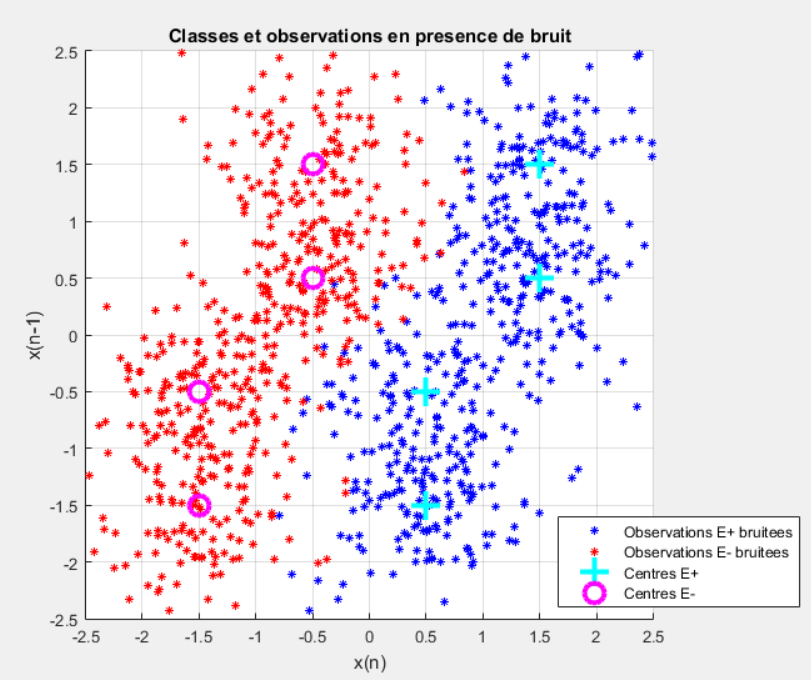
\includegraphics[width=0.85\textwidth]
    {figures/part1_2/figure1.png}
    \caption{Représentation des deux classes et des
    observations bruitées dans le plan d'observation.}
    \label{fig:classes_observations}
\end{figure}

La représentation permet de constater que les
observations bruitées se répartissent autour des
centres non bruités de leurs classes respectives.
Le bruit gaussien provoque une dispersion des points
autour de ces centres.

Cette représentation permet également d'observer
le recouvrement éventuel des deux classes, qui peut
être à l'origine des erreurs de classification.

%=========================================================
\subsection{Visualisation de la frontière de décision bayésienne}
%=========================================================

La frontière de décision bayésienne correspond à
l'ensemble des points de l'espace d'observation pour
lesquels les probabilités a posteriori des deux classes
sont égales.

Elle est définie par :

\begin{equation}
\boxed{
\partial E=
\left\{
\mathbf{x}\in\mathbb{R}^{2}
\mid P_+(\mathbf{x})=P_-(\mathbf{x})
\right\}.
}
\end{equation}

Cette frontière sépare les deux régions de décision :

\begin{itemize}
    \item Dans la première région,
    $P_+(\mathbf{x})>P_-(\mathbf{x})$ :
    l'observation est affectée à la classe $E^+$.

    \item Dans la deuxième région,
    $P_-(\mathbf{x})>P_+(\mathbf{x})$ :
    l'observation est affectée à la classe $E^-$.
\end{itemize}

\subsubsection{Approximation numérique de la frontière}

En pratique, l'égalité exacte entre les deux probabilités
est difficile à obtenir sur une grille numérique.
On utilise donc une tolérance $\epsilon$ pour identifier
les points suffisamment proches de la frontière :

\begin{equation}
\boxed{
|P_+(\mathbf{x})-P_-(\mathbf{x})|<\epsilon.
}
\end{equation}

Dans notre simulation, nous avons choisi :

\begin{equation}
\epsilon=0.001.
\end{equation}

L'espace d'observation bidimensionnel est discrétisé
sous forme d'une grille. Pour chaque point de cette
grille, les probabilités $P_+$ et $P_-$ sont calculées
à partir des expressions précédentes.

On définit alors la différence :

\begin{equation}
\Delta P(\mathbf{x})=
P_+(\mathbf{x})-P_-(\mathbf{x}).
\end{equation}

La frontière de décision correspond à la courbe de
niveau zéro de cette différence :

\begin{equation}
\boxed{\Delta P(\mathbf{x})=0.}
\end{equation}

\subsubsection{Code MATLAB}

\begin{verbatim}
% Discretisation de l'espace d'observation
nb_points = 250;

x1 = linspace(xmin,xmax,nb_points);
x2 = linspace(ymin,ymax,nb_points);

[X1,X2] = meshgrid(x1,x2);

% Construction de la grille
X_grid = [X1(:)'; X2(:)'];

nb_grille = size(X_grid,2);
P_grid = zeros(2,nb_grille);

% Calcul des probabilites sur la grille
for n = 1:nb_grille

    dist_plus = sum(bsxfun(@minus, ...
        X_plus,X_grid(:,n)).^2,1);

    dist_minus = sum(bsxfun(@minus, ...
        X_minus,X_grid(:,n)).^2,1);

    logw_plus = -dist_plus/(2*sigma2);
    logw_minus = -dist_minus/(2*sigma2);

    max_plus = max(logw_plus);
    max_minus = max(logw_minus);

    logp_plus = max_plus + ...
        log(sum(exp(logw_plus-max_plus)));

    logp_minus = max_minus + ...
        log(sum(exp(logw_minus-max_minus)));

    max_global = max(logp_plus,logp_minus);

    a = exp(logp_plus-max_global);
    b = exp(logp_minus-max_global);

    P_grid(1,n) = a/(a+b);
    P_grid(2,n) = b/(a+b);

end

% Difference entre les deux probabilites
difference_P = P_grid(1,:)-P_grid(2,:);

% Remise sous forme de matrices 2D
DIFF = reshape(difference_P,size(X1));

% Detection des points proches de la frontiere
epsilon = 0.001;
masque_frontiere = abs(DIFF)<epsilon;
\end{verbatim}

\subsubsection{Affichage de la frontière}

La commande \texttt{contour} permet de tracer la courbe
de niveau zéro de la différence entre les deux
probabilités. Les points satisfaisant le critère de
proximité à la frontière sont également représentés.

Les observations bruitées et les centres non bruités
sont superposés à cette représentation afin de faciliter
l'interprétation géométrique.

\begin{verbatim}
figure(2);
clf;
hold on;

% Frontiere theorique : P+ = P-
contour(X1,X2,DIFF,[0 0], ...
        'k','LineWidth',2);

% Points proches de la frontiere
plot(X1(masque_frontiere), ...
     X2(masque_frontiere), ...
     'g.','MarkerSize',12);

% Observations bruitees de E+
plot(X(1,indices_affiches_plus), ...
     X(2,indices_affiches_plus), ...
     'b*','MarkerSize',4);

% Observations bruitees de E-
plot(X(1,indices_affiches_minus), ...
     X(2,indices_affiches_minus), ...
     'r*','MarkerSize',4);

% Centres non bruites
plot(X_plus(1,:),X_plus(2,:), ...
     'c+','MarkerSize',16,'LineWidth',3);

plot(X_minus(1,:),X_minus(2,:), ...
     'mo','MarkerSize',12,'LineWidth',3);

grid on;
axis equal;

xlabel('x(n)');
ylabel('x(n-1)');

title(sprintf('Frontiere bayesienne : sigma2 = %.2f',sigma2));

legend('Frontiere P+ = P-', ...
       'Points |P+ - P-| < epsilon', ...
       'Observations E+ bruitees', ...
       'Observations E- bruitees', ...
       'Centres E+', ...
       'Centres E-', ...
       'Location','best');

xlim([xmin xmax]);
ylim([ymin ymax]);

hold off;

fprintf('Nombre de points proches de la frontiere : %d\n', ...
        sum(masque_frontiere(:)));
\end{verbatim}

\subsubsection{Résultat graphique et interprétation}

La figure suivante représente la frontière de décision
bayésienne obtenue pour une variance du bruit égale à
$\sigma_v^2=0.2$.

\begin{figure}[H]
    \centering
    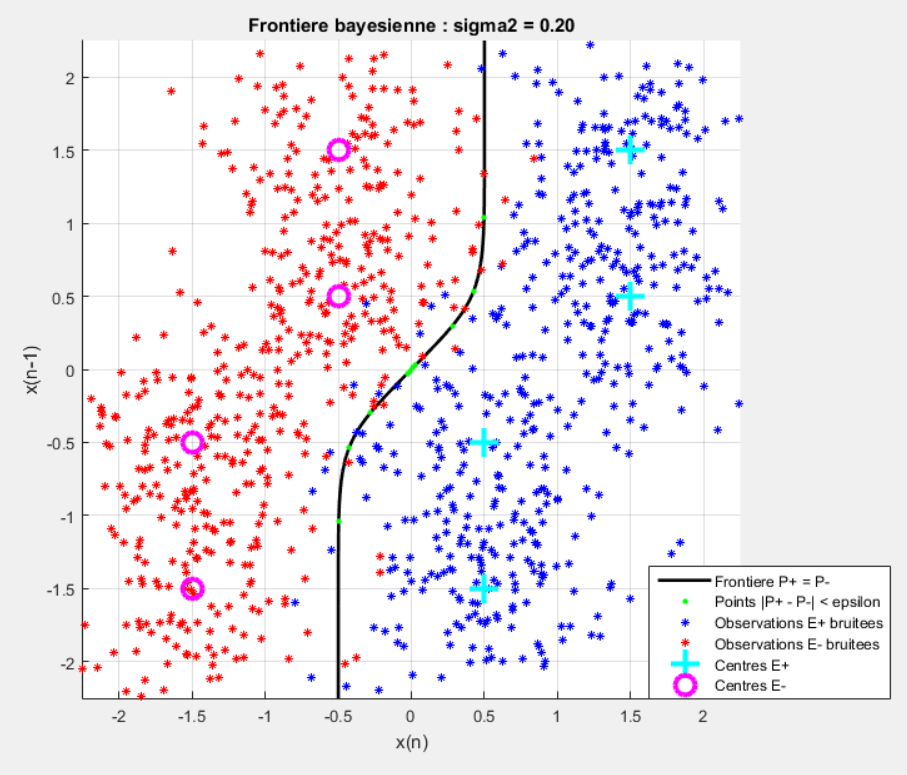
\includegraphics[width=0.9\textwidth]
    {figures/part1_2/figure2.png}
    \caption{Frontière de décision bayésienne et points
    proches de l'égalité des probabilités a posteriori.}
    \label{fig:frontiere_bayesienne}
\end{figure}

La courbe noire représente la frontière de décision,
définie par l'égalité :

\begin{equation}
P_+(\mathbf{x})=P_-(\mathbf{x}).
\end{equation}

Les points verts correspondent aux points de la grille
pour lesquels la différence absolue entre les deux
probabilités est inférieure à la tolérance choisie :

\begin{equation}
|P_+(\mathbf{x})-P_-(\mathbf{x})|<0.001.
\end{equation}

Le programme a détecté :

\begin{equation}
\boxed{
N_{\mathrm{points\ proches}}=10.
}
\end{equation}

Ce nombre correspond aux points de la grille qui
satisfont le critère numérique de proximité. Il dépend
donc de la résolution de la grille et de la valeur de
$\epsilon$. Il ne représente pas le nombre total de
points de la frontière théorique.

La courbe de niveau zéro constitue une représentation
directe de la frontière bayésienne. Elle permet de
visualiser la séparation entre les régions dans
lesquelles les observations sont affectées à $E^+$
ou à $E^-$.

